\section*{Anhang}
\label{anhang}
\addcontentsline{toc}{section}{Anhang}

\appendix

\subsection*{ContactController.java}

\begin{lstlisting}[language=java]
@RestController
@RequestMapping("/contacts")
@CrossOrigin(origins = "*")
@Api(tags = {SwaggerConfig.CONTACT_TAG})
public class ContactController {

    private static final Logger logger = LoggerFactory.getLogger(ContactApplication.class);

    private final ContactService contactService;

    public ContactController(ContactService contactService) {
        this.contactService = contactService;
    }

    @GetMapping
    @ApiOperation(value = "Get all Contacts.")
    List<Contact> getAllContacts() {
        logger.debug("GET /contacts");
        return contactService.getAllContacts();
    }

    @PostMapping
    @ResponseStatus(HttpStatus.CREATED)
    @ApiOperation(value = "Save new Contact.")
    Contact saveContact(@RequestBody Contact newContact) {
        logger.debug("POST /contacts");
        try {
            return contactService.saveContact(newContact);
        } catch (ConstraintViolationException exception) {
            throw new BadRequestException(exception.getMessage());
        }
    }

    @GetMapping("/{id}")
    @ApiOperation(value = "Get Contact by ID.")
    Contact getContact(@PathVariable String id) {
        logger.debug("GET /contacts/{}", id);
        return contactService.getContact(id)
                .orElseThrow(() -> new ResourceNotFoundException(id));
    }

    @PutMapping("/{id}")
    @ApiOperation(value = "Replace Contact by ID with new Contact.")
    Contact replaceContact(@PathVariable String id, @RequestBody Contact newContact) {
        logger.debug("PUT /contacts/{}", id);
        return contactService.replaceContact(id, newContact);
    }

    @DeleteMapping("/{id}")
    @ApiOperation(value = "Delete Contact by ID.")
    @ResponseStatus(HttpStatus.NO_CONTENT)
    void deleteContact(@PathVariable String id) {
        logger.debug("DELETE /contacts/{}", id);
        contactService.deleteContact(id);
    }

}
\end{lstlisting}

\clearpage
\subsection*{ContactServiceImpl.java}

\begin{lstlisting}[language=java]
@Service
public class ContactServiceImpl implements ContactService {

    private static final Logger logger = LoggerFactory.getLogger(ContactApplication.class);

    private final ContactRepository contactRepository;

    public ContactServiceImpl(ContactRepository contactRepository) {
        this.contactRepository = contactRepository;
    }

    @Override
    public List<Contact> getAllContacts() {
        logger.debug("Find all contacts");
        return contactRepository.findAllByOrderByLastNameAscIdAsc();
    }

    @Override
    public Optional<Contact> getContact(String id) {
        logger.debug("Find contact {}", id);
        return contactRepository.findById(id);
    }

    @Override
    public Contact saveContact(Contact newContact) {
        logger.debug("Save new contact");
        return contactRepository.save(newContact);
    }

    @Override
    public Contact replaceContact(String id, Contact newContact) {
        logger.debug("Replace contact {}", id);
        return getContact(id)
                .map(contact -> {
                    contact.setFirstName(newContact.getFirstName());
                    contact.setLastName(newContact.getLastName());
                    contact.setGender(newContact.getGender());
                    contact.setEmail(newContact.getEmail());
                    contact.setDateOfBirth(newContact.getDateOfBirth());
                    contact.setPhoneNumber(newContact.getPhoneNumber());
                    contact.setAddress(newContact.getAddress());
                    return saveContact(contact);
                })
                .orElseThrow(() -> new ResourceNotFoundException(id));
    }

    @Override
    public void deleteContact(String id) {
        logger.debug("Delete contact {}", id);
        contactRepository.deleteById(getContact(id).orElseThrow(() -> new ResourceNotFoundException(id)).getId());
    }

    @Override
    public void deleteAllContacts() {
        logger.debug("Delete all contacts");
        contactRepository.deleteAll();
    }

}
\end{lstlisting}

\clearpage
\subsection*{Frontend Interaktionen}

\begin{figure}[H] 
    \centering
    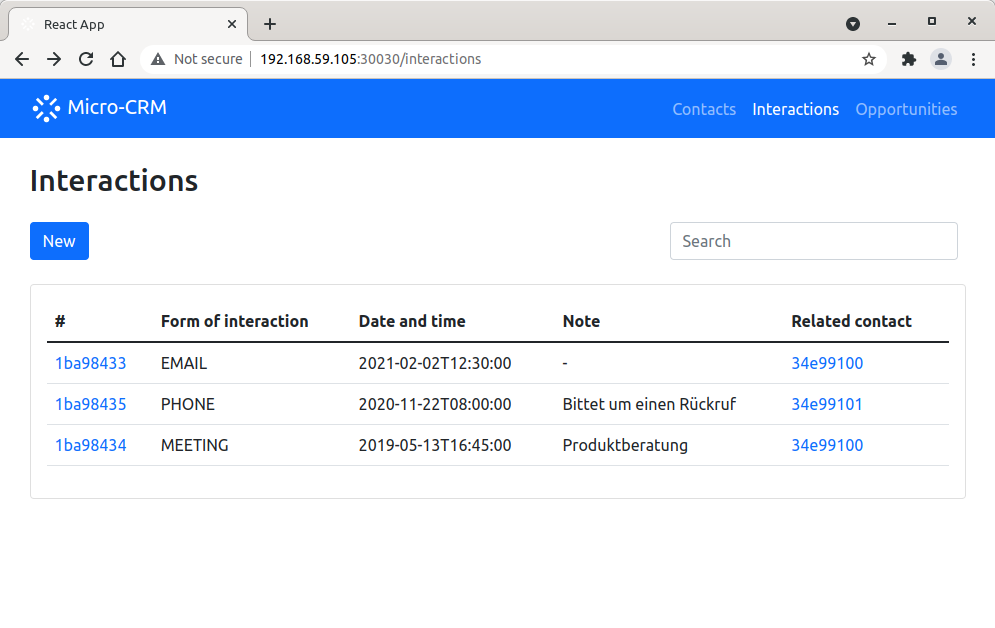
\includegraphics[width=0.9\textwidth]{figures/FrontendInteraktionen.png}
\end{figure}

\clearpage
\subsection*{Frontend Interaktion}

\begin{figure}[H] 
    \centering
    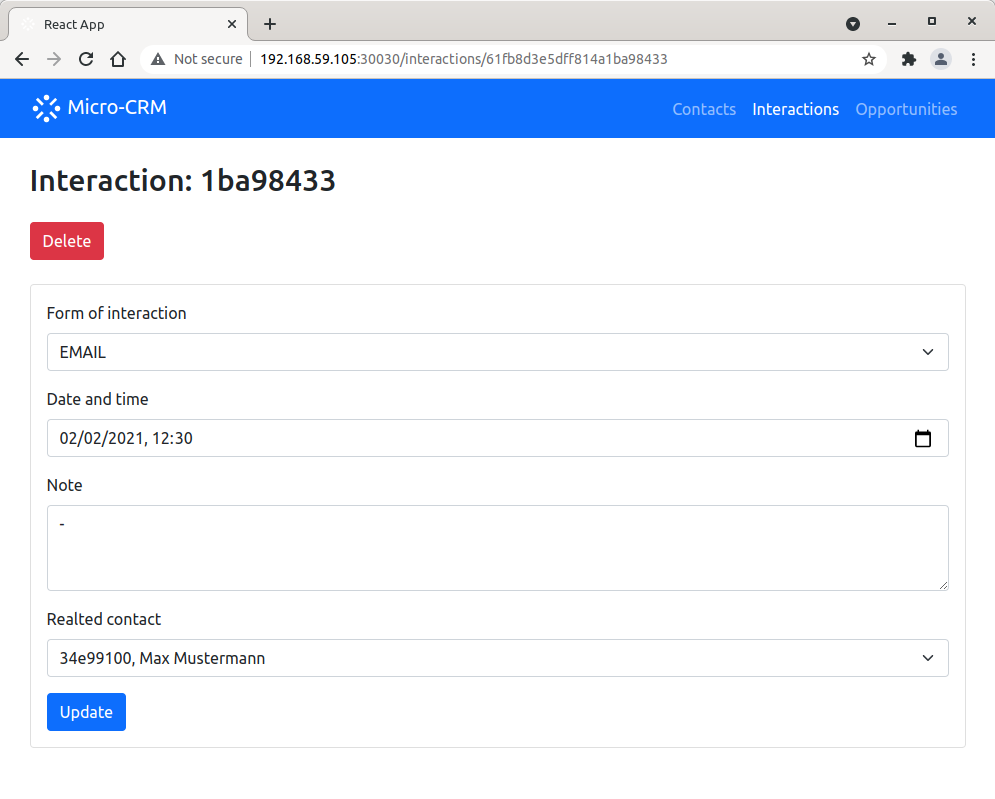
\includegraphics[width=0.9\textwidth]{figures/FrontendInteraktion.png}
\end{figure}

\clearpage
\subsection*{Frontend Kontakt}

\begin{figure}[H] 
    \centering
    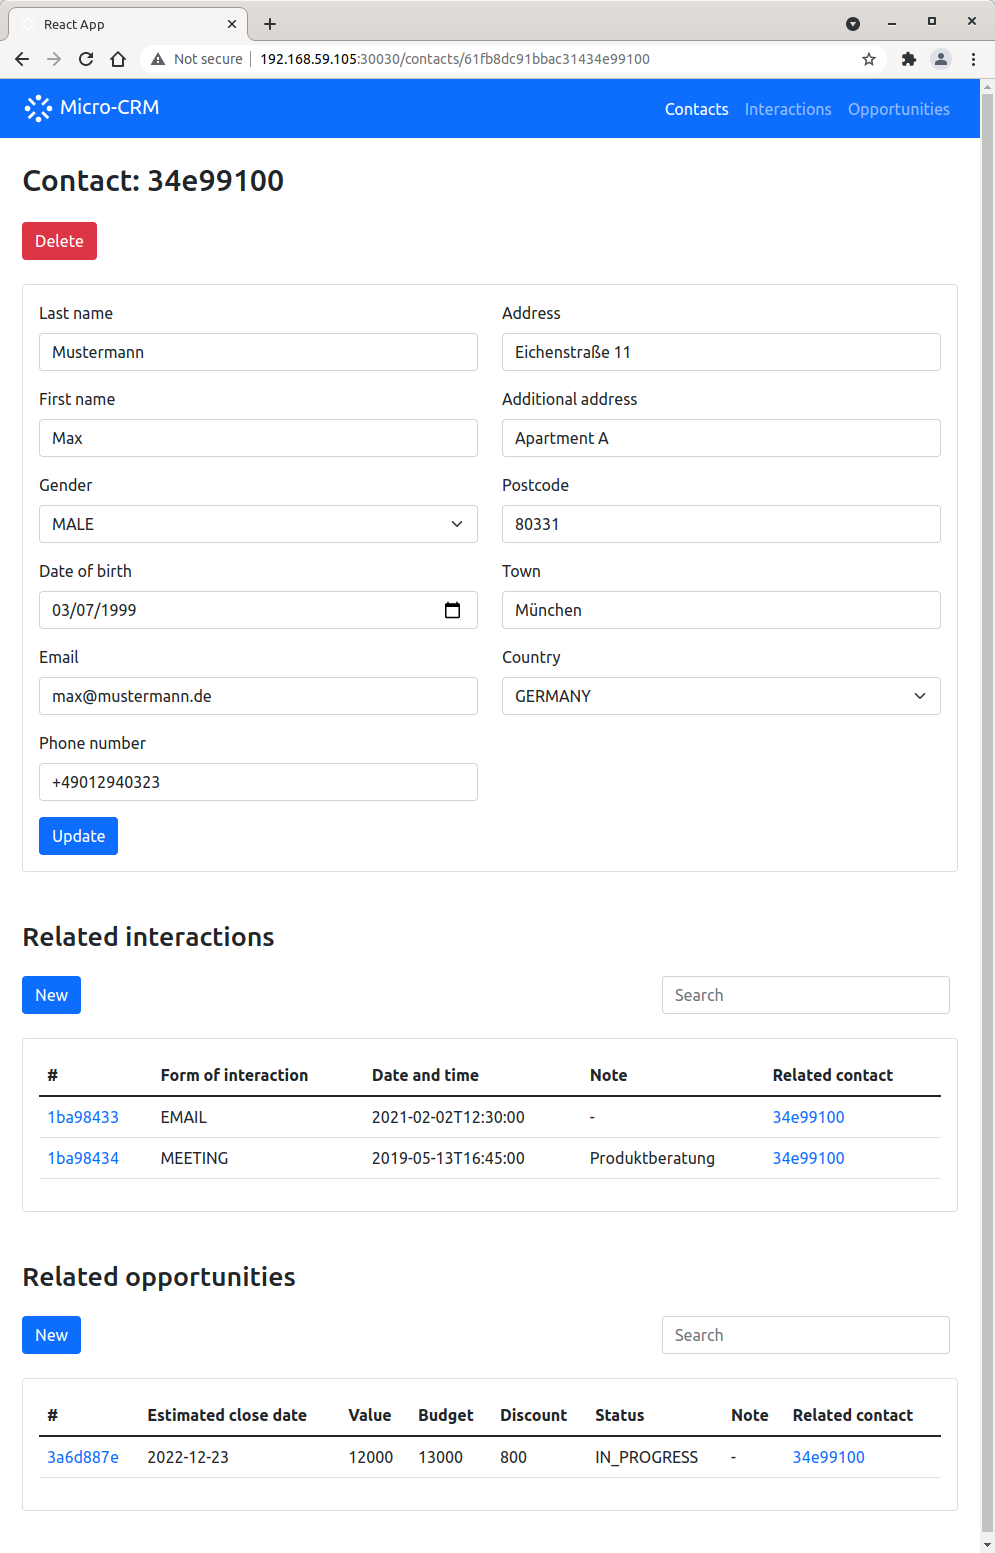
\includegraphics[width=0.85\textwidth]{figures/FrontendKontakt.png}
\end{figure}

\clearpage
\subsection*{Frontend Service-Klasse für Kontakt}
\begin{lstlisting}[language=JavaScript]
import axios from "axios";

const BACKEND = process.env.REACT_APP_BACKEND;

const CONTACT_API = 'http://' + BACKEND + (BACKEND === 'localhost' ? ':8080' : ':30010') + '/contacts';

class ContactService {

    getAllContacts() {
        return axios.get(CONTACT_API);
    }

    saveContact(contact) {
        return axios.post(CONTACT_API, contact);
    }

    getContact(id) {
        return axios.get(CONTACT_API + "/" + id);
    }

    replaceContact(id, contact) {
        return axios.put(CONTACT_API + "/" + id, contact);
    }

    deleteContact(id) {
        return axios.delete(CONTACT_API + "/" + id)
    }

}

export default new ContactService()
\end{lstlisting}

\clearpage
\subsection*{minikube Dashboard}

\begin{figure}[H] 
    \centering
    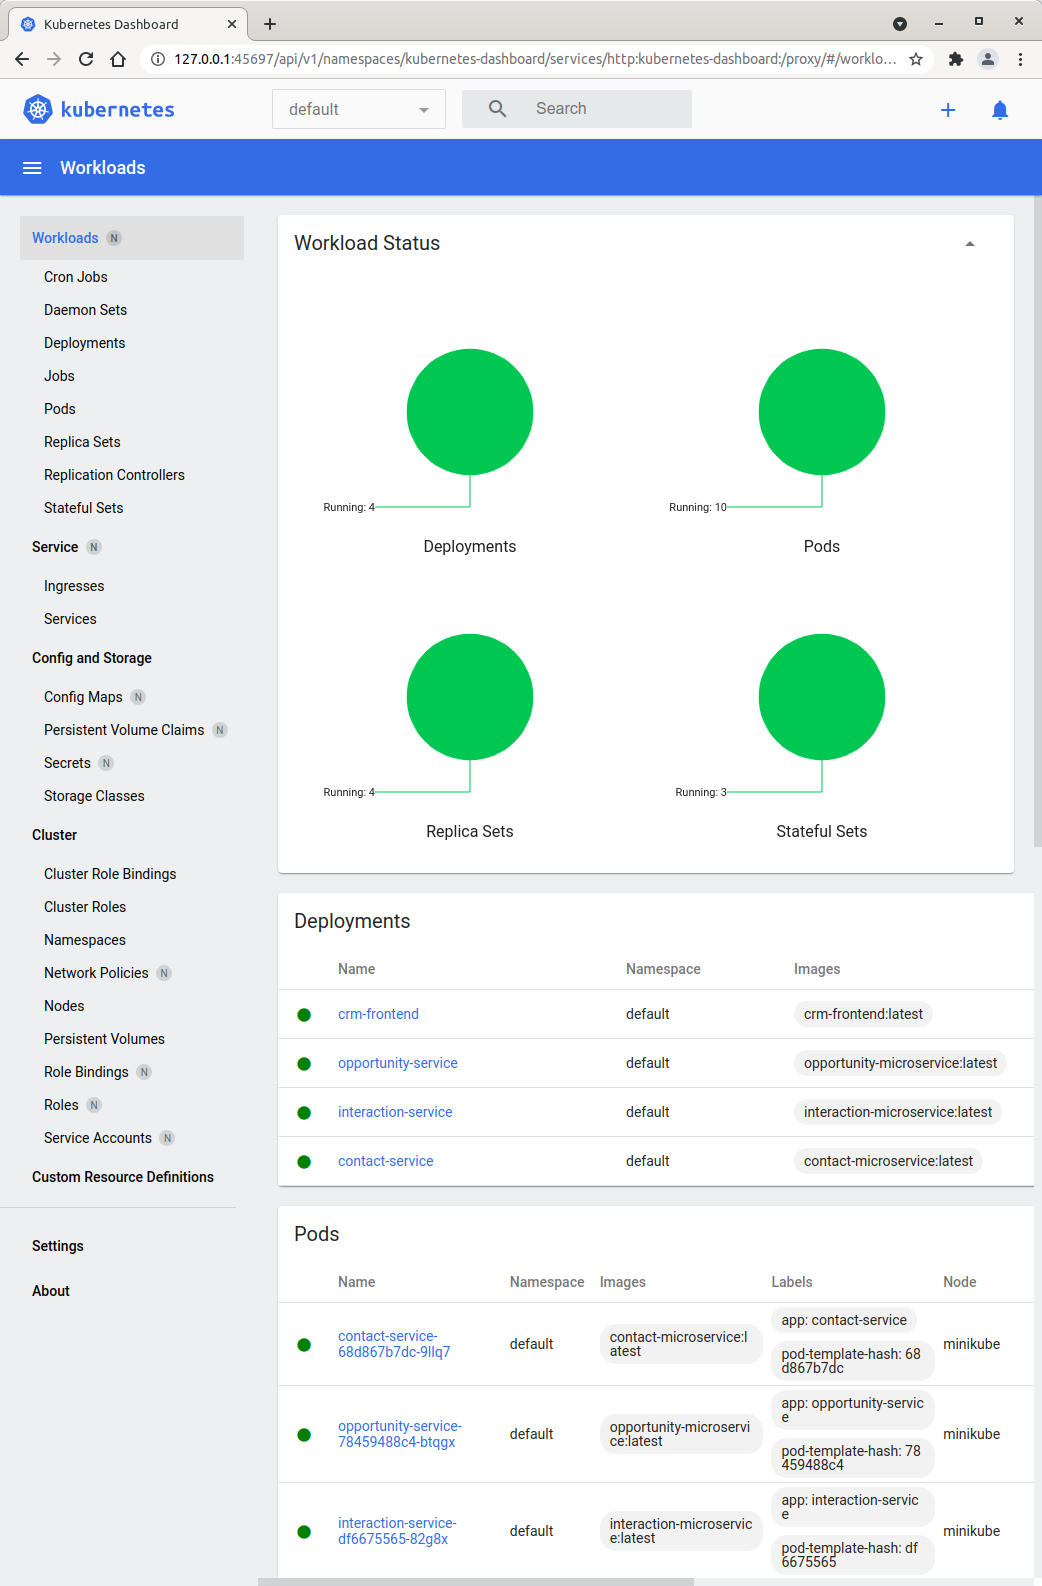
\includegraphics[width=0.855\textwidth]{figures/MinikubeDashboard.png}
\end{figure}